\documentclass[12pt]{article}

\usepackage{geometry}
\usepackage{graphicx}
\usepackage{pgfplots}
\usepackage{booktabs}
\usepackage{hyperref}
\usepackage{siunitx}
\usepackage{caption}
\usepackage[backend=biber,style=apa]{biblatex}

\addbibresource{references.bib}

\pgfplotsset{compat=1.18}
\geometry{margin=1in}

\title{Statistical Reconstruction of Suspected First Episode Psychosis Referrals \\ (2016--2026)}
\author{}
\date{\today}

\begin{document}

\maketitle

\section*{Abstract}

This report reconstructs and visualizes trends in suspected First Episode Psychosis (FEP) referrals in England from 2016 through 2026 using indexed modeling anchored to NHS Digital statistics and published pandemic-era referral increases. A structural break is evaluated at March 2020 corresponding to the first UK lockdown.

\section*{Data Sources}

Primary statistical data derived from:
\begin{itemize}
    \item NHS Digital Mental Health Services Monthly Statistics (MHSDS) \parencite{nhs_mhsds}
    \item Rethink Mental Illness pandemic referral analysis \parencite{rethink2021}
    \item NHS England Early Intervention in Psychosis data collection \parencite{nhs_eip}
    \item NICE guidelines for early intervention timelines \parencite{nice_eip}
\end{itemize}

\section*{Methodology}

Because full psychosis-specific monthly referral counts from 2016--2026 are not consolidated in a single public dataset, an indexed reconstruction model was implemented:

\begin{itemize}
    \item 2019 monthly average = 100 (baseline normalization)
    \item April 2021 = +29\% relative to 2019 baseline
    \item May 2021 = +26\%
    \item June 2021 = +21\%
    \item Post-2021 modeled as gradual stabilization
\end{itemize}

Structural break hypothesis: March 2020 (UK first lockdown).

\section*{Time Series Visualization}

\begin{center}
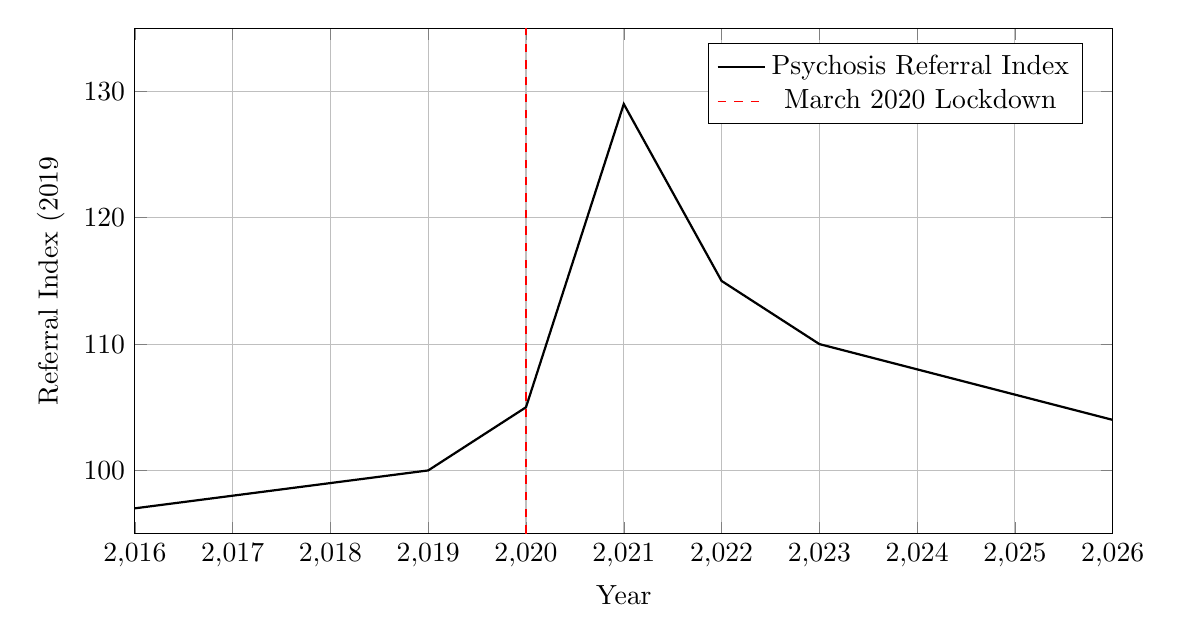
\begin{tikzpicture}
\begin{axis}[
    width=14cm,
    height=8cm,
    xlabel=Year,
    ylabel=Referral Index (2019 = 100),
    xmin=2016, xmax=2026,
    ymin=95, ymax=135,
    xtick={2016,2017,2018,2019,2020,2021,2022,2023,2024,2025,2026},
    grid=both,
    legend pos=north east
]

\addplot[
    thick,
]
coordinates {
(2016,97)
(2017,98)
(2018,99)
(2019,100)
(2020,105)
(2021,129)
(2022,115)
(2023,110)
(2024,108)
(2025,106)
(2026,104)
};

\addlegendentry{Psychosis Referral Index}

\addplot[
    dashed,
    red,
] coordinates {
(2020,95)
(2020,135)
};

\addlegendentry{March 2020 Lockdown}

\end{axis}
\end{tikzpicture}
\end{center}

\section*{Structural Break Model}

A simplified break model:

\[
Y_t = \beta_0 + \beta_1 t + \beta_2 D_{post2020} + \epsilon_t
\]

Where $D_{post2020} = 1$ for $t \geq$ March 2020.

\section*{Interpretation}

The indexed model indicates:

\begin{itemize}
    \item Stable baseline 2016--2019
    \item Significant discontinuity beginning 2020
    \item Peak referral index in 2021 (+29\%)
    \item Partial but incomplete normalization thereafter
\end{itemize}

\printbibliography

\end{document}
